\documentclass{beamer}
\usepackage{graphicx}
\usepackage{booktabs} % For better table rules
\usepackage{amsmath} % For math symbols
% Choose a theme
\usetheme{Madrid}


\title{Decoding Student Retention and Churn of Vodafone (Telecel) in KNUST}
\subtitle{A Survival Analysis Approach}
\author{Musah Faridu Oubda
	\\ Kassim Asana
	\\ Sarpong Linda
	\\ Torsi Edmond Collins
	\\ Asiamah Ezekiel}
\begin{figure}
	\centering
	
\includegraphics[width=0.3\linewidth]{logo.png}
\end{figure}
\institute{Kwame Nkrumah University of Science and Technology}
\date{\today}

\begin{document}
	% Title page
	\begin{frame}
		\titlepage
	\end{frame}
	
	% Table of contents
	\begin{frame}{OUTLINE}
		\tableofcontents
	\end{frame}
	
	
	\section{INTRODUCTION}
	
	\begin{frame}
		\frametitle{BACKGROUND OF STUDY}
		\begin{itemize}
			
			
			\item 	The Ghanaian telecommunications industry, particularly Vodafone (now Telecel), faces significant challenges with customer churn. Retaining customers is crucial for profitability, especially in a highly competitive market where acquiring new customers is more expensive than retaining existing ones.
			\item 	
			Telecel, which acquired Vodafone in early 2023, aims to enhance service offerings and improve customer retention. The study focuses on understanding and addressing student churn at KNUST using survival analysis methods to develop strategies for reducing churn and improving customer satisfaction.
			
		\end{itemize}
	\end{frame}
	
	\begin{frame}
		\frametitle{PROBLEM STATEMENT}
		\begin{itemize}
			\item Student churn persists due to a lack of understanding of the factors driving churn and retention. 
			\item This research aims to identify these factors and develop strategies to improve retention rates using survival analysis models.
			
			
		\end{itemize}
	\end{frame}
	
	\begin{frame}
		\frametitle{RESEARCH OBJECTIVES}
		\begin{itemize}
			\item Main Objective: Analyze student retention and churn using survival analysis
			\item Specific Objectives:
			\begin{itemize}
				\item Identify factors influencing churn
				\item Analyze demographic patterns
				\item Evaluate churn rates for different services
				\item Assess impact of network quality on retention
			\end{itemize}
		\end{itemize}
	\end{frame}
	
	\section{Methodology}
	
	
	
	\begin{frame}
		\frametitle{METHODOLOGY}
		\begin{itemize}
			\item 
			The data was collected via a survey, capturing specific aspects relevant to the study while ensuring confidentiality and ethical consideration
			\item The sample size was determined through cluster sampling, targeting approximately 768 students from a population of about 85,000, with each of the 6 clusters representing different colleges within KNUST having around 128 students each.
			
			
		\end{itemize}
	\end{frame}
	
	\begin{frame}
		\frametitle{METHODOLOGY}
		\begin{itemize}
			\item The data preprocessing involved examining the dataset for missing data and handling it to ensure completeness and representativeness for analysis. Categorical variables were transformed into numeric format using label encoding with Python.
			\item The dataset was then organized to facilitate essential components like time duration, event indicators, and relevant covariates.
			
		\end{itemize}
	\end{frame}
	
	\begin{frame}
		\frametitle{METHODOLOGY (CON'T)}
		\begin{itemize}
			\item Kaplan-Meier Estimator is a
			non-parametric method used to estimate the survival function from lifetime data.
			\item Cox Proportional Hazards Model (Cox PH) is a semi-parametric model that relates the time until an event occurs to one or more covariates.
			\item Accelerated Failure Time (AFT) Model is estimates how covariates accelerate or decelerate the time to event.
			\item Akaike Information Criterion (AIC) helps in model selection by balancing model fit and complexity. A lower AIC indicates a better fit. 
			\item Concordance Index measures a model's ability to rank predictions accurately. A higher C-index indicates better predictive ability.
		\end{itemize}
	\end{frame}
	
	\begin{frame}
		\frametitle{DATA DESCRIPTION AND ANALYSIS}
		\begin{itemize}
			
			
			\item \textbf{Demographic information:}
			
			Gender, college, and residence
			\item \textbf{Event of interest and duration}
			
			Churn and Level
			\item \textbf{Services Used:}
			
			Voice call, mobile data and sms texting
			\item \textbf{Factors influence discontinuation: }
			
			Multiple networks, network coverage, customer service, data allowance, high cost of services
			\item \textbf{Data Activity:}
			
			Data usage, exhaust monthly data
		\end{itemize}
	\end{frame}
	
	
	
	\section{Analysis and Findings}
	\begin{frame}
		\frametitle{KAPLAN  MEIER}
		\begin{figure}[H]
			\centering
			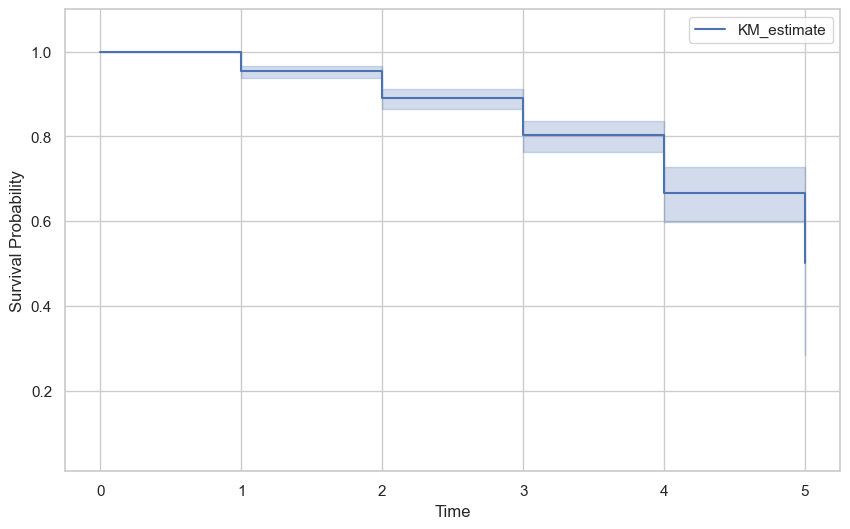
\includegraphics[width=0.47\textwidth]{Figure 4/4.1.png}
			\hfill
			\caption{KM Curve}
			\label{Table 1}
			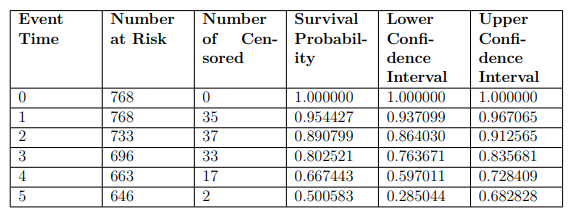
\includegraphics[width=0.47\textwidth]{Presentation/ana.png}
			
			\caption{KM Analysis}
			\label{Figure 1}
		\end{figure}
	\end{frame}
	
	
	\begin{frame}
		\frametitle{ANALYSIS AND FINDINGS}
		\begin{figure}
			\centering
			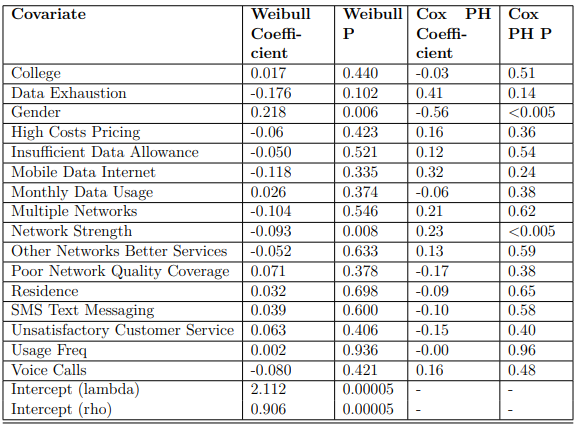
\includegraphics[width=0.5\linewidth]{Presentation/cox and weilbull.png}
			\caption{Cox and Weibull}
			\label{Figure 2}
		\end{figure}
	\end{frame}
	
	
	\begin{frame}
		\frametitle{ANALYSIS AND FINDINGS CON'T}
		\begin{figure}[H]
			\centering
			\begin{minipage}{0.48\textwidth}
				\centering
				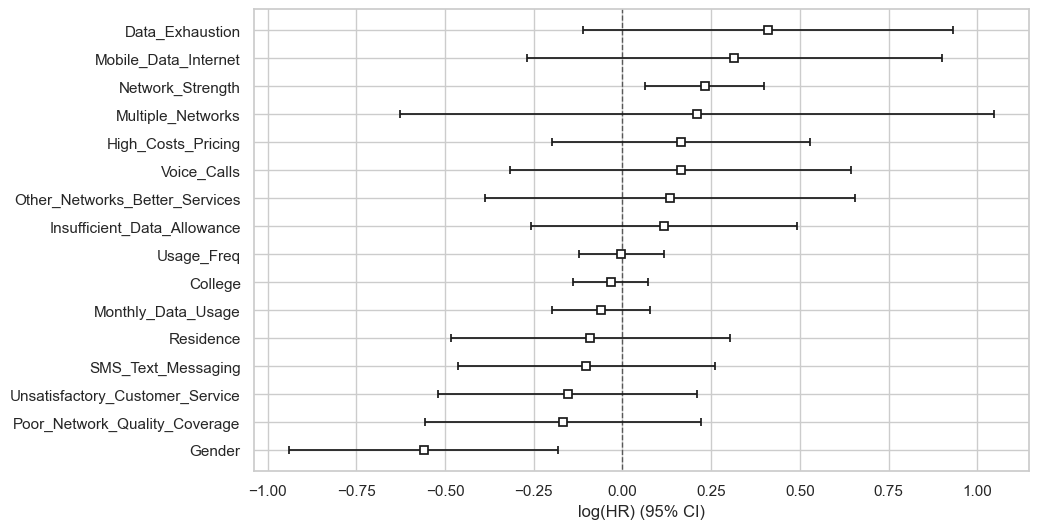
\includegraphics[width=\textwidth]{Figure 4/4.2.png}
				\caption{Cox Coefficients}
				\label{Figure 3}
			\end{minipage}\hfill
			\begin{minipage}{0.48\textwidth}
				\centering
				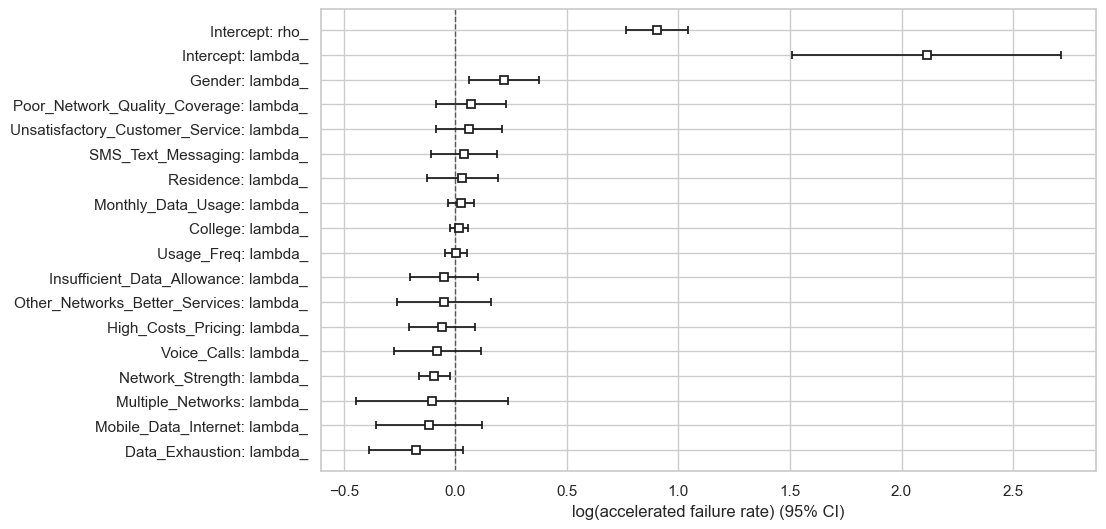
\includegraphics[width=\textwidth]{Figure 4/4.4.png}
				\caption{Weibull Coefficients}
				\label{Figure 4}
				
			\end{minipage}
		\end{figure}
	\end{frame}
	
	
	\begin{frame}
		\frametitle{MODEL COMPARISON}
		%Table here
		\begin{table}[H]
			\centering
			\begin{tabular}{lcc}
				\toprule
				\textbf{Model} & \textbf{Concordance} & \textbf{AIC} \\
				\midrule
				Weibull & 0.624 & 815.516 \\
				Cox PH & 0.62 & 1479.47 \\
				\bottomrule
			\end{tabular}
			\caption{Model Concordance and AIC values}
			\label{Table 2}
			
		\end{table}
		
	\end{frame}
	
	\section{Conclusion}
	
	\begin{frame}
		\frametitle{SUMMARY OF FINDINGS}
		\begin{itemize}
			\item The research shows that Weibull AFT is the best model for both prediction and fit.
			\item  High service costs, poor network coverage, and inadequate customer support drive churn. Competitive pricing, reliable network coverage, and responsive customer service improve retention.
			\item Data services have the highest churn rates thus indicating students' high value on reliable data. services.
			\item Younger students and those in their final year show higher churn rates. Gender differences are minimal and thus do not greatly affect churn rates.
		\end{itemize}
	\end{frame}
	
	\begin{frame}
		\frametitle{RECOMMENDATIONS}
		\begin{itemize}
			\item Increase the monthly data usage as most students to 10G.
			\item Enhance the quality and reliability of network coverage across KNUST to reduce churn rates.
			\item Improve the responsiveness and quality of customer support to address student concerns more effectively.
			\item Implement competitive pricing strategies and introduce loyalty programs to retain students.
			
		\end{itemize}
	\end{frame}
	
	\begin{frame}
		\frametitle{Conclusion}
		\centering{ THANK YOU}
		
		
		
	\end{frame}
	
\end{document}

